% !TEX root = set_recommendation.tex
% \section{Modeling desiderata}
% \label{sec:desiderata}
% Our goal is to build a recommendation model that provably maximizes an
% evaluation metric. The model should also approximate other models that recommend
% items based on sets of attributes. We propose criteria for models that rank from
% sets, and then exhibit a model satisfying these desiderata:
% \begin{itemize}
% \item Order-invariance: if the input to the model includes an unordered set of
%   attributes, the output of the model should not depend on the order that the
%   set elements are fed to the model.
% \item Improved recall: training the model should provably improve the evaluation
%   metric of recall. Models that satisfy this desideratum make good recommenders.
%   (In contrast, it is unclear whether a model that reconstructs the training
%   data well will lead to maximum recall performance.)
% \item Universal approximation: the model should be able to approximate any other
%   order-invariant model. This reduces the need to compare to other models in
%   lieu of comparing parameterizations of a single model.
% \item Parameter-sharing: the model should share parameters across items with
%   similar sets of attributes. This enables the model to scale to large
%   real-world datasets.
% \end{itemize}
% The criterion of order-invariance is necessary due to the set-valued features
% associated with every item. The parameter-sharing desideratum further narrows
% the set of models and guides the development of architectures parameterizing a
% model. The desiderata of improved recall and universal approximation, if
% satisfied, frees practitioners to focus on building architectures for a single
% model. Intra-model comparisons, rather than arduous inter-model comparisons,
% enable the development of generic architectures that work across many datasets
% for ranking from sets.
\section{The rankfromsets model}
\label{sec:rankfromsets}

% !TEX root = ../set_recommendation.tex
\begin{figure*}[t!]
  \centering
%  \pdfimageresolution=500  
  \includegraphics[width=0.95\textwidth]{fig/arxiv_user_embeddings_tsne.png}
  \caption{\label{fig:arxiv_tsne} \acrlong{rfs} trained on arXiv reading
    behavior clusters researchers by their most frequently-read arXiv category
    (best viewed in color). On this data, \acrlong{rfs} is trained to recommend
    items using their attributes as described in \Cref{sec:experiments_arxiv};
    the set of attributes for a paper is the set of words in the abstract. A
    visualization of the user embeddings in the inner product regression
    function in \Cref{eqn:rankfromsets} yields an interpretable map of science.
    We use the t-SNE algorithm~\citep{maaten2008visualizing} for visualizing the
    high-dimensional embeddings in two dimensions. In this map of science,
    fields of study are related according to patterns in how people read papers
    in neighboring fields. Each marker represents a user embedding; the color
    assigned to a user is determined the user's most-read arXiv category. The
    color assigned to a category is determined by the most-read categories
    across the arXiv, with similar colors assigned to similar fields according
    to the arXiv ontology. For an interactive version of this map, please visit
    anon-url which enables zoom and display of all 143 arXiv category labels to
    explore the relationships between different fields of science.}
\end{figure*}


%%% Local Variables:
%%% mode: latex
%%% TeX-master: "../set_recommendation"
%%% End:


\acrlong{rfs} is a recommendation model that recommends items with attributes to
users. Let $u \in \{1, \ldots, N\}$ be a user, $m \in \{1, \ldots, M\}$ be an
item, and $\yum~\in~\{0,1\}$ be a binary indicator where $1$ indicates user $u$
consumed item $m$. For each item $m$, there is an associated set of attributes
$x_m \in \{0,1\}^{|V|}$ from a vocabulary of $V$ attributes.

We assume that a recommendation model is given a budget of $K$ recommendations
to be made for each user. In response, the recommender system produces a list of
$K$ distinct recommendations $\mathbf{r}_u = (r_{u1}, \ldots, r_{uK})$ for each
user. The goal of the recommendation task in this paper is to maximize the
expected recall,
\begin{equation}
\label{eqn:recall}
\text{Recall@}K = \mathbb{E}_u\left[\frac{\sum_{r \in \mathbf{r}_u} y_{ur}}{\sum_{m} \yum}\right] \, ,
\end{equation}
where the expectation is over all users in the empirical data distribution
$\cD$. \acrfull{rfs} combines three techniques to maximize \Cref{eqn:recall}.
First, we cast recommendation as a classification task. Second, we learn user-
and attribute-level embeddings. Statistical strength is shared between items
with similar attributes by representing items as the mean of their attribute
embeddings. Third, we scale \gls{rfs} to large datasets by using a stochastic
optimization-based negative sampling training procedure to fit the model.

\subsection{Recommendation through classification}
\label{subsec:rankfromsets:classification}
\acrfull{rfs} casts the recommendation problem as a classification task. Given a
user-item pair $(u,m)$, \gls{rfs} learns to predict the probability that item
$m$ will be consumed by user $u$,
\begin{equation}
\label{eqn:prob_y_given_um}
p(\yum = 1 | u, m) = \sigma\left( f \left(u, x_m\right) \right) \, ,
\end{equation}
where $x_m$ is the set of attributes associated with item $m$ and $\sigma$ is
the sigmoid function. The recommendations made by \gls{rfs} are the maximum
likelihood set,
\begin{equation}
\label{eqn:argmax}
\mathbf{r}_u(K) = \underset{\mathbf{r} \in \mathbb{N}^K}{\text{argmax}} \sum_{m\in\mathbf{r}} f \left( u, x_{m} \right) \, .
\end{equation}
% Setup the problem here as a generic classification problem. the recommendations are going to be the argmax over the probabilities output by a classifier.

To motivate treating recommendation as classification, we make the following observation.
\begin{proposition}
\label{prop:maximizing-recall}
Let $u \in \mathcal{U}$ be a user, $x \in \mathcal{X}$ be an item, and
$y(u,x) \in \{0,1\}$ be an indicator of whether user $u$ logged item $x$. Let
$\mathcal{E}$ be the worst-case error for binary classifier $\hat{y}(u,x)$ on
any $(u,x)$ pair drawn from the data $\mathcal{D}$,
\begin{equation*}
  \mathcal{E} = \max_{(u, x) \in \mathcal{D}} \mbone\left[ \hat y(u, x) \neq y(u, x) \right] \, .
\end{equation*}
A binary classifier with zero worst-case error ($\mathcal{E}=0$) maximizes
recommendation recall.
\end{proposition}
\begin{proof}
  A model with zero worst-case error is a perfect classifier: it assigns greater
  probability to positively-labeled datapoints than to negatively-labeled
  datapoints. In other words, it ranks positive examples above negative
  examples. Recall in \Cref{eqn:recall} is measured by the fraction of
  positively-labeled items in a ranking returned by the model. In a classifier
  that achieves zero worst-case error, positively-labeled datapoints must be
  ranked higher than other datapoints, maximizing recall.
\end{proof}

\Cref{prop:maximizing-recall} is simple, but conceptually important. Under the
assumption that a perfect classifier exists, a consistent method for learning a
classifier will be a consistent method for learning a recommendation system that
targets expected recall. In practice, as with any regression method, a perfect
classifier is unachievable. \Cref{prop:maximizing-recall} is a guiding principle
rather than a finite-sample guarantee of maximal performance. As we show in
\Cref{sec:experiments}, the classification approach of \gls{rfs} performs well
in practice.

\subsection{Embedding users and items}
\label{subsec:rankfromsets:embeddings}
For recommending items with attributes, \Cref{prop:maximizing-recall} says that
building a classifier such as \acrlong{rfs} is optimal if we measure
recommendation performance with recall. To parameterize the \gls{rfs}
classifier, we need to choose a regression function $f(u, x_m)$.
A straightforward parameterization is an inner product,
\begin{equation}
\label{eqn:rankfromsets}
  f\left(u, x_m\right) = \theta_u^\top\left(\frac{1}{|x_m|}\sum_{j\in x_m}
  \beta_j + g(x_m)\right) + h(x_m) \, .
\end{equation}
Each element in the inner product regression function in \Cref{eqn:rankfromsets}
has an intuitive interpretation:
\begin{itemize}
\item The user embedding $\theta_u \in \mathbb{R}^d$ captures the latent
  preferences for user $u$. This captures the individual-level tastes of a user
  and is analogous to the user preference vector in classical collaborative
  filtering or the row embedding in matrix factorization.
\item The attribute embedding $\beta_j \in \mathbb{R}^d$ is the latent quality
  conveyed through item $m$ having attribute $j$. The set $x_m$ contains only
  attributes with $x_{mj}=1$. Attributes that are not associated with item $m$
  are ignored.
\item The item embedding function $g(x_m) \in \mathbb{R}^d$ captures qualities
  not conveyed through the set of item attributes. This term in the regression
  function enables collaborative filtering by capturing unobserved patterns in
  item consumption such as popularity. We describe how to construct this
  function below.
\item The item intercept function $h(x_m) \in \mathbb{R}$ makes an item more or
  less likely simply due to availability.
\end{itemize}

\paragraph{Scalable item embedding and item intercept functions} The
parameterization of the item embedding function $g(x_m)$ depends on the size of
the data. If the number of items is small, $g$ can function as a lookup for
unique intercepts for every item. However, if the number of items is so large
that unique item intercepts lead to overfitting, we need a scalable
parameterizations of item embeddings $g$ using additional information about
every item. For example, if the data consists of foods in meals, we can define a
meal intercept as the mean of food intercepts, yielding a scalable item
intercept function. The item intercept function $h(x_m)$ that maps item
attributes to scalars is constructed in the same way. We study both of these
choices in \Cref{sec:experiments}.

The inner product regression function in \Cref{eqn:rankfromsets} has several
benefits. It requires computing a sum over only the attributes each item is
associated with. This enables \gls{rfs} to scale to large attribute vocabularies
where traditional matrix factorization methods are intractable. Second, the
embed-and-sum approach to set modeling is provably flexible. We describe deep
variants of \gls{rfs} and detail how \gls{rfs} can approximate other
recommendation models in the next section.
% Consider the example from \Cref{sec:introduction} of predicting whether a user
% would enjoy a meal. Each user has some preferences about which meals they enjoy.
% A meal is made up of foods or attributes. One does not need to consider foods
% that are not in a meal; unused foods can be ignored. In addition, a meal is more
% than its foods. For instance, a user trying to eat healthier may enjoy all the
% ingredients in a meal, but if it is deep fried, it will be unappealing. The
% regression function in \gls{rfs} should be able to learn such latent patterns in
% meal consumption. Finally, even if a meal is not very appealing to a user, it
% may be popular and available everywhere, making it more likely to be consumed.

% The regression function $f(u, x_m)$ parameterizes the generative process of the
% labels conditional on the item attributes and user,
% $\yum \sim \textrm{Bernoulli}\left(\yum; \sigma(f(u, x_m)\right)$.

% Specifically, recent results in deep learning for set-valued data show that
% such an approach is sufficient to model nearly any function
% \cite{DBLP:journals/corr/ZaheerKRPSS17}. In theory, it may be necessary to
% apply a nonlinearity, such as a deep neural network, to $f$ to learn any
% function. In preliminary experiments, we found increasing the embedding size
% $d$ in the embedding model offered a better tradeoff between parameter size
% and model performance than the additional parameters added by a neural
% network.

\subsection{Deep extensions}

The \gls{rfs} inner product regression function in \Cref{eqn:rankfromsets} is a
log-bilinear model. But there are several other choices of regression function,
and we draw on the deep learning toolkit for classification to build two other
example architectures. With finite data and finite compute, one architecture
will outperform another, or prove insufficiently flexible to capture patterns in
user consumption. The optimal choice of architecture depends on computational
tradeoffs. We conclude this section by showing that in the regime of infinite
data and compute, all the \gls{rfs} architectures we propose, including the
inner product, can approximate other recommendation models that operate on
set-valued input such as matrix factorization.

\paragraph{Parameterizing \gls{rfs} using a neural network} As an alternative to
the log-bilinear model in \Cref{eqn:rankfromsets}, we can use a deep neural
network as a regression function:
\begin{align}
  f\left(u, x_m\right) = \phi\left(\theta_u, \frac{1}{|x_m|}\sum_{j\in x_m}
  \beta_j, g(x_m)\right) + h(x_m) \, ,
  \label{eqn:neural-network}
\end{align}
where the deep network $\phi$ has weights and biases and takes as inputs the
user embedding, sum of attribute embeddings, and item intercept. Such a neural
network can represent functions that may or may not include the inner product in
\Cref{eqn:rankfromsets} (\emph{ex~ante}, it is unclear whether a finite-depth,
finite-width neural network can represent the inner product).

% This contrasts
% the inner product regression function: \emph{ex~ante}, it is unclear whether a
% finite-depth, finite-width neural network can represent the inner product in
% \Cref{eqn:rankfromsets}.

\paragraph{Parameterizing \gls{rfs} with a residual network} Another possibility
of regression function for \gls{rfs} is a combination of
\Cref{eqn:rankfromsets,eqn:neural-network}, using an idea borrowed from deep
residual networks for image classification~\citep{he2015deep}. In this
architecture a neural network $\phi$ with the same inputs as in
\Cref{eqn:neural-network} is used to learn the residual in the inner product
model:
\begin{align}
  f\left(u, x_m\right) = \theta_u^\top\left(\frac{1}{|x_m|}\sum_{j\in x_m}
  \beta_j + g(x_m)\right) + \phi + h(x_m) \, .
  \label{eqn:residual}
\end{align}

\paragraph{The choice of regression function in \gls{rfs} depends on the data}
On finite data, with finite compute, one parameterization of \gls{rfs} will
outperform another. To demonstrate this, we simulated synthetic data from the
same generative process \gls{rfs} employs with a ground-truth regression
function (a square kernel), and found that the residual and deep
parameterizations outperformed the inner product architecture. These results are
included in \Cref{sec:simulation}, and motivate exploring other architectures
than the three examples we give.

\subsection{Generalization property}
\label{subsec:method:generalization}
If we take a step back from the setting of finite data and compute, a bigger
picture emerges, which reveals the choice of regression function in \gls{rfs}
does not matter. Any \gls{rfs} architecture is sufficiently flexible to
approximate other recommendation models that operate on set-valued input. Before
deriving this result, we first describe the class of recommendation models that
operate on set-valued input.

\paragraph{\gls{rfs} and multiple matrix factorization are examples of
  permutation-invariant models} The regression function $f$ in \gls{rfs}
operates on set-valued input: the unordered collection of item attributes $x_m$.
A set is, by definition, permutation-invariant: it remains the same if we
permute its elements. Functions that operate on set-valued inputs must also be
permutation-invariant. \gls{rfs} is permutation-invariant as the set of
attributes associated with an item enter into
\Cref{eqn:rankfromsets,eqn:neural-network,eqn:residual} via summation. Other
examples of permutation-invariant models are matrix factorization,
recommendation models based on word embeddings, and permutation-marginalized
recurrent neural networks. We show these models are permutation-invariant and
evaluate them in \Cref{sec:experiments}.

\paragraph{\gls{rfs} can approximate other permutation-invariant
  models such as matrix factorization} We apply a theorem from
\citet{zaheer2017deep} to show that \gls{rfs} can approximate
other recommendation models. 

\begin{proposition}
  Assume the vocabulary of attributes (set elements) is countable,
  $\lvert V \rvert < \lvert \bbN_0 \rvert$. \acrshort{rfs} can approximate any
  permutation-invariant recommendation model.
  \label{prop:universal-approximation}
\end{proposition}
The proof follows directly from Theorem~2 in \citet{zaheer2017deep} and we will
not restate it here. (The only change to the proof is the mapping from set
elements to one-hot vectors,
$c \colon V \to \left\{0, 1\right\}^{\lvert V \rvert}$ to yield a unique
representation of every object in the powerset.)


\Cref{prop:universal-approximation} means that any of the parameterizations in
\Cref{eqn:rankfromsets,eqn:neural-network,eqn:residual} are flexible enough to
approximate other principled recommendation models that leverage item
attributes, such as content-based matrix
factorization~\cite{gopalan2014content-based}. This proposition also supports
exploring other parameterizations of \gls{rfs} that may have better
computational or statistical properties.

\subsection{Stochastic optimization}
\label{subsec:rankfromsets:negative-sampling}

The parameters for \acrlong{rfs} are learned by stochastic optimization. Denote
the full set of \gls{rfs} model parameters by $\mbgamma$, and let~$\cD_u$~be the
empirical data distribution for a user. Let $\lambda_u$ be a reweighting
parameter. The maximum likelihood objective for \gls{rfs} is
\begin{equation}
  \label{eq:objective}
  \begin{aligned}
  \cL(\mbgamma, \lambda_u) = \E_u\big[ \E_{x_m \sim \cD_u \mid \yum = 1}\left[\log p(\yum =1 \mid x_m; \mbgamma)\right] \\
  - \lambda_u \E_{x_k \sim \cD_u \mid \yuk = 0}[\log p(\yuk = 0 \mid x_k; \mbgamma)]
                \big] \\
  \end{aligned}
\end{equation}

In traditional regression, altering the ratio of positive to negative examples
by reweighting leads to inconsistent parameter estimation. The inconsistency
stems from the randomness in the labels, given the features. However, recall in
\Cref{eqn:recall} assumes that each user, item attribute set pair ($u, x_m$)
uniquely determines whether the item was consumed or not (the label $\yum$).
Here, all reweightings produce the same result. This means that for any negative
example weight $\lambda_u$, the learned model will be the same. In practice we
set $\lambda_u$ to balance the positive and negative examples for each user. We
use stochastic optimization to maximize \Cref{eq:objective}. We describe two
negative sampling schemes that are dependent on the choice of evaluation metric.
% for a single datapoint $(x_m, \yum=1)$ is
% \begin{align}
% \begin{split}
%   \cL(\theta, & (x_m, \yum), \{(x_k, \yuk)\}) =\\
%   &\log p(\yum = 1 \mid x_m; \theta) + \sum_{k=1}^L \log p(\yuk = 0 \mid x_k;
%   \theta),\\
%   &\textrm{with}~x_k\sim\textrm{Uniform}(I).
%   \label{eq:objective}
% \end{split}
% \end{align}

% As users only interact with a small number of items, this objective function is
% dominated by negatively-labeled datapoints with~$\yum = 0$. We use stochastic
% optimization to maximize \Cref{eq:objective} and learn parameters jointly.
% Stochastic optimization requires subsampling the terms in the objective with
% negative labels. Such subsampling directly leads to a binary classification
% binary classification loss function with negative samples, as in previous work
% on word embeddings~\cite{mikolov2013distributed} and recommender
% systems~\cite{he2017neural,song2018neural}.
% The \gls{rfs} parameterization in
% \Cref{eqn:prob_y_given_um,eqn:argmax,eqn:rankfromsets} is bi-convex and could be
% fit through alternating coordinate descent. That is, fixing the user embeddings,
% the problem is convex in each of the other parameters; similarly, the problem is
% convex in the user parameters if the other parameters are fixed. For each
% coordinate in the user step, such a procedure would require iterating over all
% items. The massive number of items in the datasets in \Cref{sec:experiments}
% makes this intractable; similar issues could also arise for datasets with many
% users.

% \paragraph{Negative sampling} All observed positive labels (i.e. instances where
% $\yum = 1$) are divided into mini-batches. For each mini-batch, each
% positively-labeled sample is paired with a negatively-labeled sample. The
% negatively-labeled sample has the same user as its paired sample, but the item
% is sampled uniformly from a set of items. This procedure is not unbiased, but
% still leads to a consistent classifier: note that any reweighting of items that
% assigns nonzero weight to all items can be arbitrarily biased, but still lead to
% a consistent classifier. As long as every item has nonzero weight, the infinite
% data limit ensures that the classifier will learn to discriminate between
% positively- and negatively-labeled datapoints. We decide to balance
% positively-labeled datapoints with negative samples in each mini-batch as it is
% easy to implement as shown in \Cref{sec:code}.
% We note that any negative sampling
% scheme that assigns nonzero weight to every item leads to a consistent
% classifier.

% Ideally, the sampling set should be the set of all items which the user has not
% consumed, where~$\yum~=~0$. But maintaining and sampling from user-specific sets
% of negative labels can be computationally prohibitive. When the item set is
% large and labels are sparse (that is, $\yum = 0$ for most user, item pairs),
% embedding models are often trained by drawing negative samples uniformly from
% the item set~\cite{mikolov2013distributed}. For training \gls{rfs}, we propose
% two different negative sampling distributions that trade off quality of the
% learned parameters for scalability of the training procedure.

%   \hspace{1.8cm}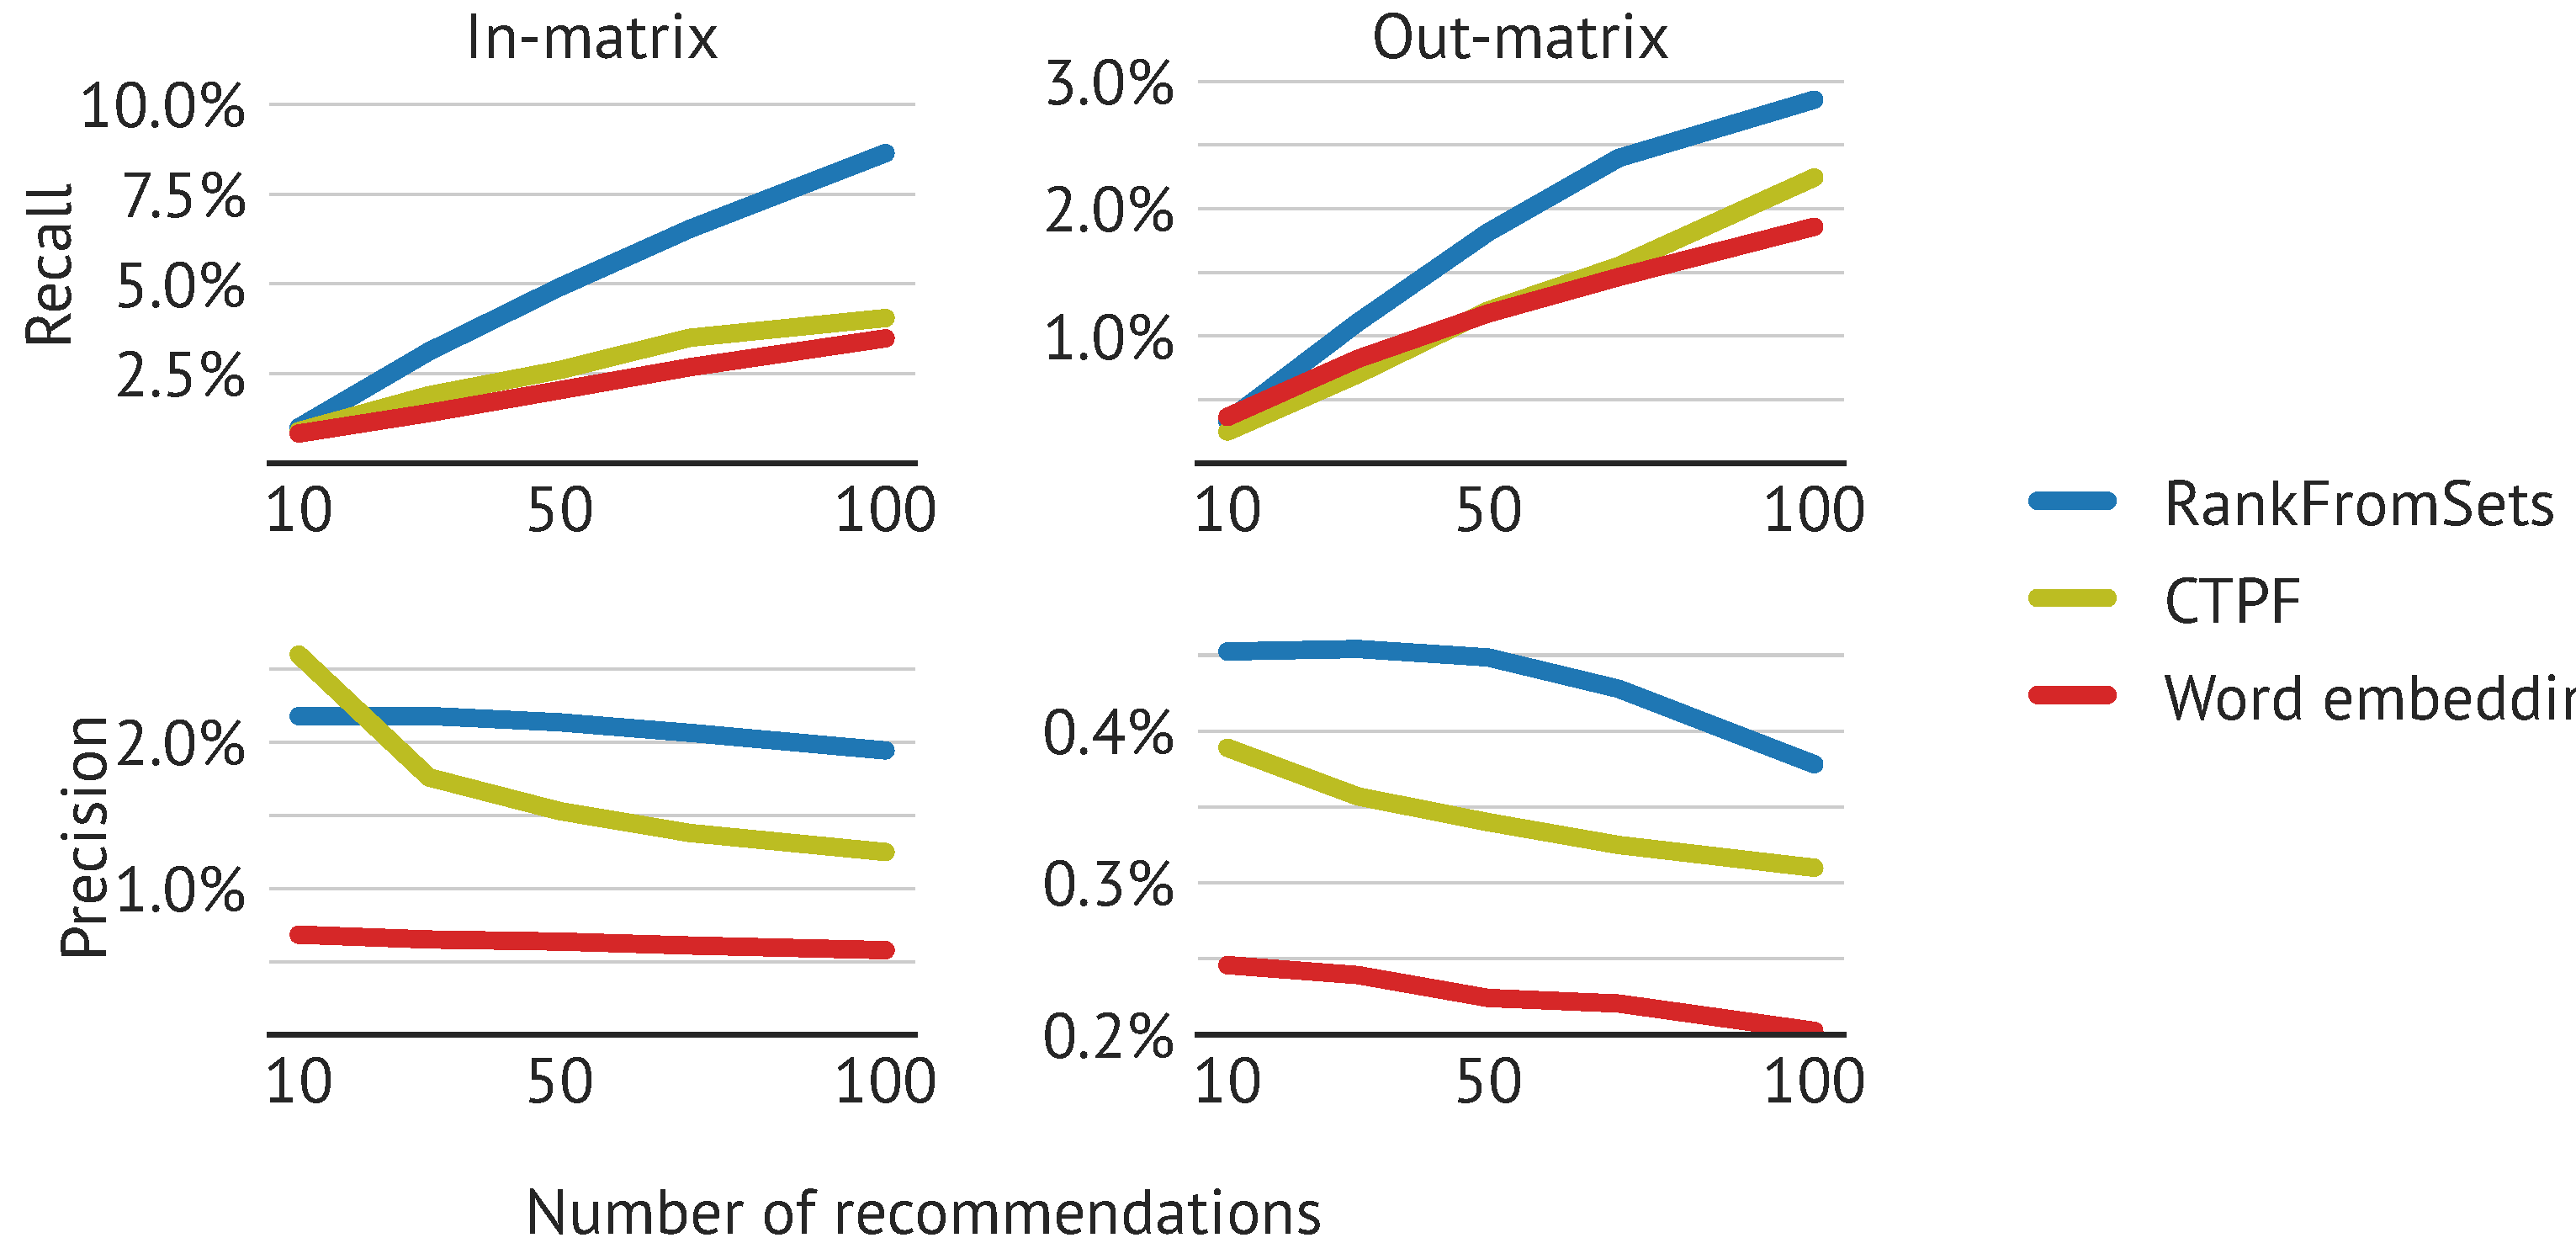
\includegraphics[width=0.7\linewidth]{fig/arxiv}
\newcommand{\mysize}{0.9in}
\newcommand{\mywidth}{0in}
\newcommand{\figwidth}{0.18\linewidth}
\begin{figure*}[t!]
  \centering
  \captionsetup[subfigure]{oneside,margin={-1cm,0cm}}
  \hspace*{\fill}%
  \begin{subfigure}[]{\figwidth}
    \centering
    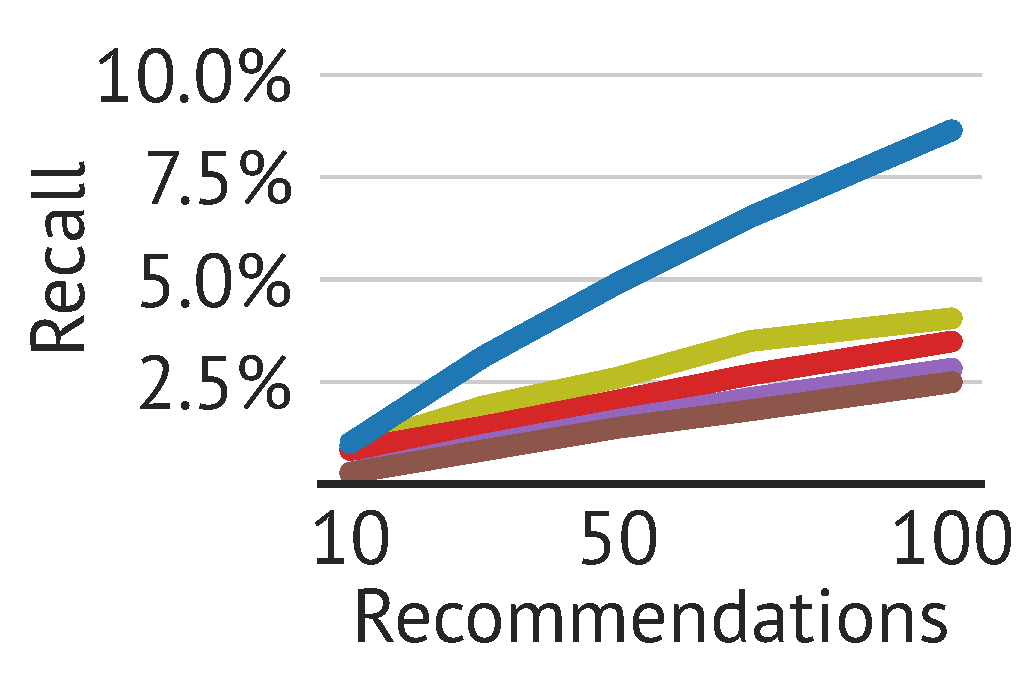
\includegraphics[height=\mysize]{fig/arxiv-in-matrix-recall}
    \caption{In-matrix recall}%
    \label{fig:arxiv-in-recall}%
  \end{subfigure}
  \hfill\hspace{\mywidth}%
  \begin{subfigure}[]{\figwidth}
    \centering
    
\includegraphics[height=\mysize]{fig/arxiv-out-matrix-recall}
    \caption{Out-matrix recall}%
    \label{fig:arxiv-out-recall}%
  \end{subfigure}
  \hfill\hspace{\mywidth}
  \begin{subfigure}[]{\figwidth}
    \centering
    
\includegraphics[height=\mysize]{fig/arxiv-in-matrix-precision}
    \caption{In-matrix precision}%
    \label{fig:arxiv-in-precision}%
  \end{subfigure}
  \hfill\hspace{\mywidth}
  \begin{subfigure}[]{\figwidth}
    \centering
    
\includegraphics[height=\mysize]{fig/arxiv-out-matrix-precision}
    \caption{Out-matrix precision}%
    \label{fig:arxiv-out-precision}%
  \end{subfigure}
  \hfill\hspace{\mywidth}
  \begin{subfigure}[]{0.1\linewidth}
    \centering
    \raisebox{14mm}{
      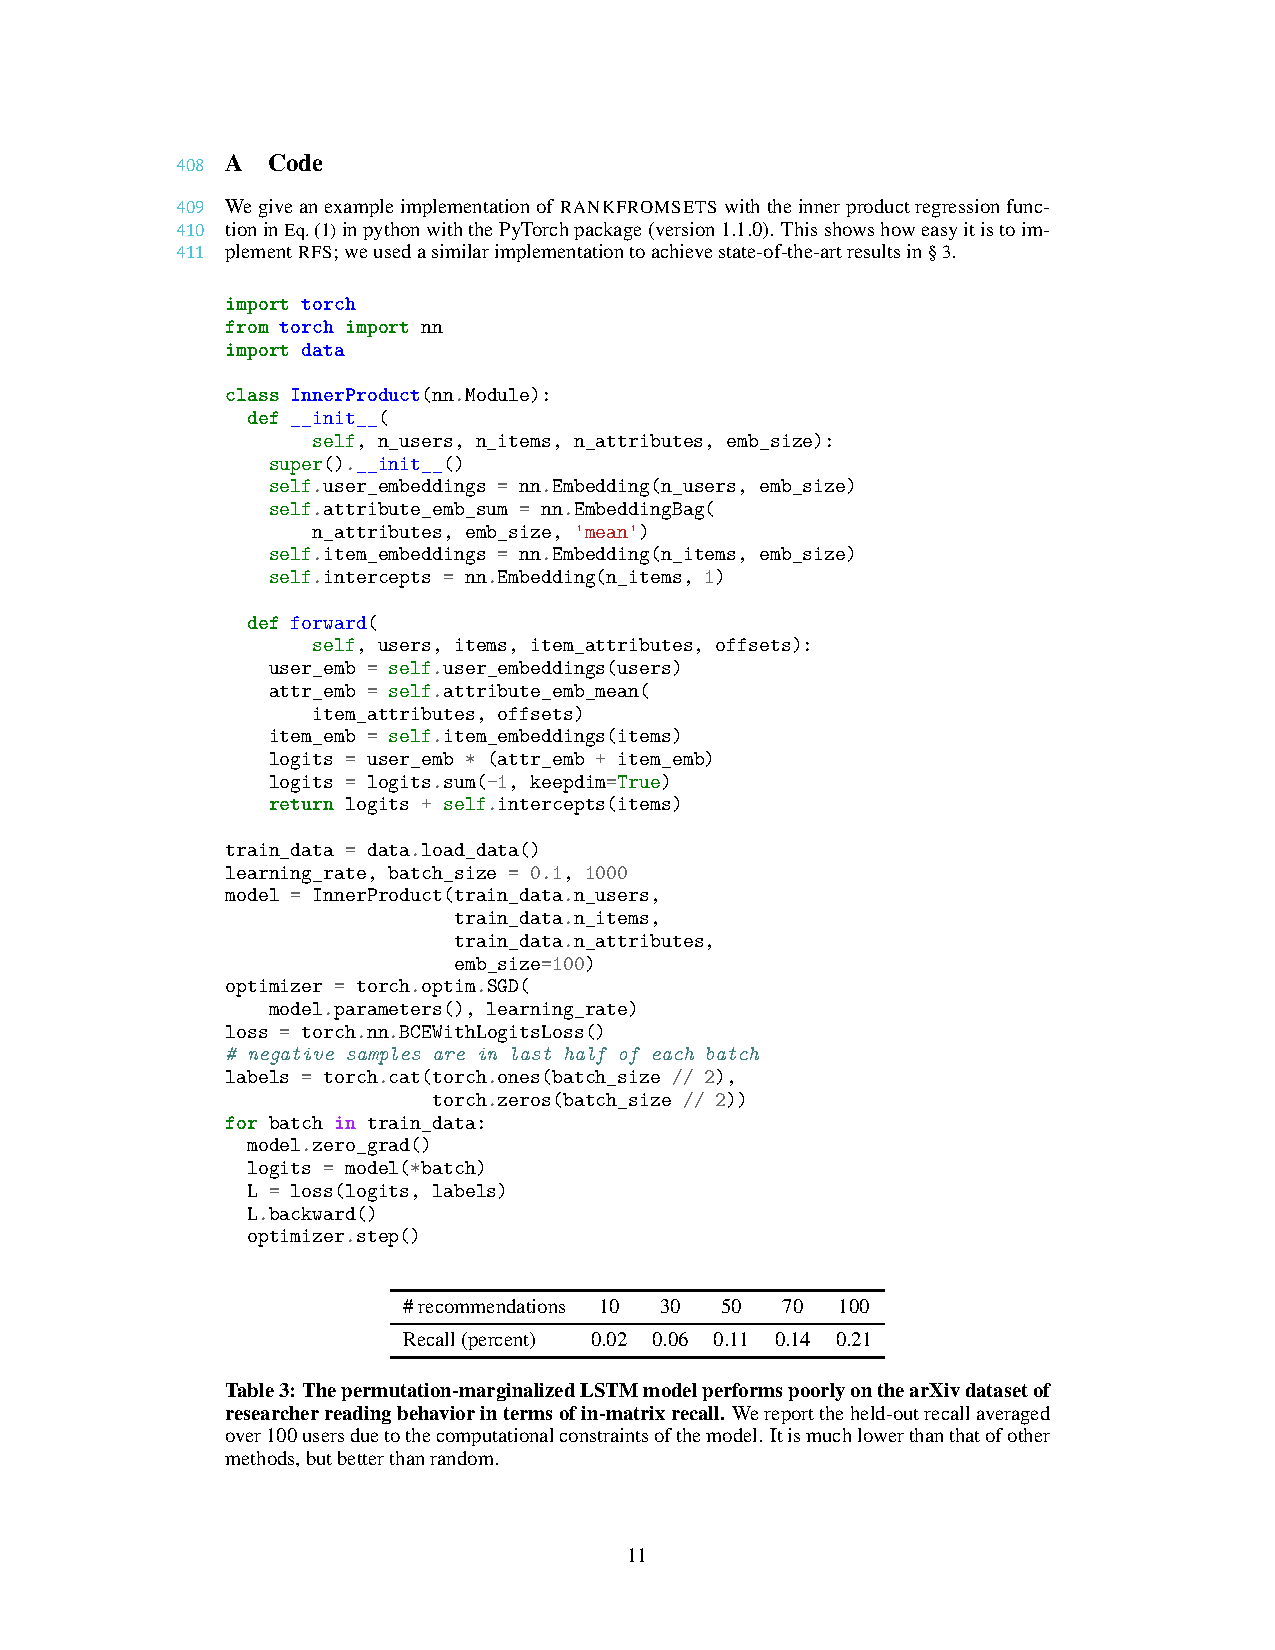
\includegraphics[width=0.9in]{fig/arxiv-legend}
    }
  \end{subfigure}
  \hspace*{\fill}%
  % \vspace{-0.5cm}
  \caption{\label{fig:arxiv-performance} \acrlong{rfs} with the inner
    product regression function in \Cref{eqn:rankfromsets} outperforms
    collaborative topic Poisson factorization (\acrshort{ctpf}, described
    in~\citet{gopalan2014content-based}) and a word embedding model on
    recommending arXiv papers to scientists. In this dataset the items are
    documents and the attributes are the unique words in the abstracts.
    Recommendation performance is evaluated using precision and recall to match
    the evaluation in \citet{gopalan2014content-based}, and these metrics are
    reported on training (in-matrix) documents and cold-start (out-matrix)
    documents with no clicks in the training set. }
\end{figure*}

%%% Local Variables:
%%% mode: latex
%%% TeX-master: "../set_recommendation"
%%% End:

\paragraph{Corpus sampling} Negative samples can be drawn uniformly over the
entire corpus of items. If the item set is large, this can be an expensive
procedure. This negative sampling scheme and resulting approximation of
\Cref{eq:objective} is similar to the objective functions in other recommender
systems~\cite{he2017neural,song2018neural}.

On large datasets, it is infeasible to calculate recall for evaluation, as
\Cref{eqn:recall} requires ranking every item for every user (e.g. in
\Cref{sec:experiments_meals} we study a dataset with over $10$M items). We
define a scalable evaluation metric based on recall, and describe how it leads
to a natural choice of negative sampling distribution.

\paragraph{Batch sampling and sampled recall} We define sampled recall as
follows. Start with held-out datapoints with positive labels, $(x_m, \yum = 1)$.
For every held-out datapoint, $K-1$ datapoints with negative labels
$(x_k, \yuk = 0)$ are sampled from the rest of the held-out data, which together
yield a set of $K$ datapoints. A recommendation model is used to rank the $K$
datapoints $r_{u1}, \ldots, r_{uK}$. Sampled recall is the fraction of the
held-out datapoints that the model ranked in the top $k$:
\begin{equation}
\begin{aligned}
\label{eq:sampled-recall}
  \textrm{Sampled}&\textrm{Recall@}k = \E_{um}\left[\frac{\sum_{r\in \{\mb{r}_{u1},
      \ldots \mb{r}_{uk}\}} y_{ur}}{K}\right] \, ,\\
\end{aligned}
\end{equation}
where the expectation is over users and items in the held-out set of datapoints.
This evaluation metric is scalable: instead of using a model to rank every item,
it requires ranking $K$ items. Sampled recall is~$1$~if~$k~=~K$, as the held-out
datapoint with $\yum = 1$ is in each list of $K$ datapoints to be ranked.
% For
% example, with $M=10$, an average sampled recall@1 of $0.5$ means for 50\% of the
% held-out datapoints, the item consumed by the user was ranked first by the model
% (out of $9$~items randomly sampled from the held-out data of other users). For
% the sampled recall metric we choose $M=10$, meaning $9$ `fake' meals are sampled
% uniformly from other users' meals in the held-out validation and test sets.

When sampled recall is used as an evaluation metric, batch sampling is a natural
way to draw negative samples. Sampled recall is calculated on items drawn from
other user's data. We define batch sampling as generating negative samples by
permuting mini-batch items. Besides corresponding to the sampled recall metric,
this technique is memory-efficient, as it requires that only the current
mini-batch be in memory.

In addition to scalability, both of the negative sampling procedures above have
the advantage of implicitly balancing the classifier. As
\citet{veitch2019empirical} note, using stochastic gradient descent with
negative sampling is equivalent to a Monte Carlo approximation of the
reweighted, or balanced, classification loss.

%%% Local Variables:
%%% mode: latex
%%% TeX-master: "set_recommendation"
%%% End:
